\documentclass[12pt]{report}
\usepackage{setspace}
%\usepackage{subfigure}

\pagestyle{plain}
\usepackage{amssymb,graphicx,color}
\usepackage{amsfonts}
\usepackage{latexsym}
\usepackage{amsmath}
\usepackage{algorithm}
\usepackage{algorithmicx}
\usepackage{algpseudocode}

\newtheorem{theorem}{THEOREM}
\newtheorem{lemma}[theorem]{LEMMA}
\newtheorem{corollary}[theorem]{COROLLARY}
\newtheorem{proposition}[theorem]{PROPOSITION}
\newtheorem{remark}[theorem]{REMARK}
\newtheorem{definition}[theorem]{DEFINITION}
\newtheorem{fact}[theorem]{FACT}

\newtheorem{problem}[theorem]{PROBLEM}
\newtheorem{exercise}[theorem]{EXERCISE}
\def \set#1{\{#1\} }

\newenvironment{proof}{
PROOF:
\begin{quotation}}{
$\Box$ \end{quotation}}


\graphicspath{
  {/home/hege/Documents/Thesis/msc-thesis/}
  {/home/hege/Documents/Thesis/msc-thesis/figures/}
}

\newcommand{\nats}{\mbox{\( \mathbb N \)}}
\newcommand{\rat}{\mbox{\(\mathbb Q\)}}
\newcommand{\rats}{\mbox{\(\mathbb Q\)}}
\newcommand{\reals}{\mbox{\(\mathbb R\)}}
\newcommand{\ints}{\mbox{\(\mathbb Z\)}}

%%%%%%%%%%%%%%%%%%%%%%%%%%


\title{  	{ 
\includegraphics[scale=.5]{ucl_logo.png}}\\
{{\Huge Project Title}}\\
{\large Optional Subtitle}\\
		}
\date{Submission date: Day Month Year}
\author{Hermanni H{\"a}lv{\"a} \thanks{
{\bf Disclaimer:}
This report is submitted as part requirement for the MSc CSML degree at UCL. It is
substantially the result of my own work except where explicitly indicated in the text.
The report may be freely copied and distributed provided the source is explicitly acknowledged
\newline  %% \\ screws it up
}
\\ \\
MSc. Computational Statistics and Machine Learning\\ \\
Supervisor: Prof. Bradley Love}

\begin{document}
 
\onehalfspacing
\maketitle
\begin{abstract}
Summarise your report concisely.
\end{abstract}
\chapter*{Acknowledgements}
\thispagestyle{empty}
I would like to\dots
\clearpage

\tableofcontents
\listoffigures
\listoftables
\setcounter{page}{1}

\chapter{Notes}
\begin{itemize}
  \item essentially our model proposes that semantic taxonomy is the best guide to visual taxonomy -- better than wikipedia 
    \item discuss how first trained on small data set
    \item mention knowledge transfer
    \item one problem is that we are training only transformation to the leafs of the nodes. I wonder if we could includ basic level labels since those are the ones humans learn first and also some suggest on average capture most distinction (see the two papers)
    \item look at yolo 9000 for wordnet explanation
    \item Do I clearly state that CNNs are the state-of-the-art on image classification, give some example of current results / super human performance or when they wont competitions first time
    \item applications of zero-shot learning and better representation. e.g. autonomous vehicles need to make deductions. 
    \item benthos example on wikipedia
    \item because of benthos problem -- it would be worth testing our model on the animals with attributes data set 
    \item Is this really zero-shot learning since we are using knowledge
    \item see DEvise for motivating ZSL
    \item one motivatin is that it's expensive to get labelled data
    \item a potential problem is dimensionality is it too low? especially we wish some local smoothness in therms of visual samples in embedding space.perhaps more dimensions are needed for this. Though hard to really say since hyperbolic space..
    \item doman adaptation to help with transfer  from leaf to centre?
    \item problem if overall visual things arent near to each other in the hierarchy. Maybe more true for animals but less true for things that are 'used' for something.
    \item maybe one contribution is that visual similarity is not entire from taxonomy e.g. zebra maybe difficult to guess. Our benefit is really probabily to predict basic level classes. 
    \item zero shot image retrieval
    \item final layer of CNN doesnt have necessarily enough detailed information contained. Perhaps need to make links to higher layers \cite{Ba2015}
    \item is projection domain shift problem for this instance where output space is structured
    \item if need information on applications of ZSL see Fu and Sigal semi-supervised vocabulary-informed learning
    \item use maybe some other data set as well
    \item some very complex architectures - we want to produce simple easily justifiable solution
\end{itemize}

\chapter{Intro/Literature Review Notes}

Imagine you have never seen a zebra, but you know what horses look like and someone tells you that Zebras are basically horses with black and white stripes. Later when you see a picture of such a creature on TV, you immediately recognize it as a Zebra even though at no point have you received a labelled data. This type of behaviour would be extremely valuable for machine vision systems. Scarcity of labels\dots. In real life application e.g. autonomous vehicles\dots


Contrast this to the performance of a typical deep learning or machine learning algorithm, it would fail unless it has received a labelled data \dots\dots.


Humans are able to extract rich semantic information from visual scenes. For instance, upon viewing a picture of a dog, we may also be able to identify it as a specific breed such as a golden retriever. Further, our understanding of the image benefits from semantic knowledge that is not captured explicitly in the visual features of a specific image. For example, we also know that the dog belongs in the category of mammals which, in turn, are animals and thus living entities. While this type of hierarchical semantic visual understanding comes to us effortlessly, it remains a challenging task for computer vision. In fact, most image classification models are trained on data sets with single, mutually exlusive labels and thus the learnt feature representations do not account, for example, for both cat and dog being four-legged animals. Why is this a problem? Generalization?  An exception to this is the area of knowledge transfer and related tasks such as zero-shot learning in which the aim is to predict labels of previously unseen classes of images; a popular approach for zero-shot learning is to borrown strength from, say text data, to create a semantic space that embed all the possible labels of images including those not seen previously. Mapping between images and the semantic space is then learned using the 'seen' images. Once this mapping is learnt, it can be used to transform previously unseen images into the semantic space and then apply some distance measure to label it as the category thats cloest in the embedding space. We postulate that the same idea could also be employed in the simple image classification tasks to achieve better generalization performance. In particular, we will train a deep learning model for image classification against a hierarchical semantic embedding derived from the WordNet database which, as we will show, will correspond to regularizing the model weights to account for these semantic relationships. We will use the recently developed poincare embeddings as the resulting embedding space can capture both the similarity between the possible labels as well as the hierarchical semantic relationships encoded by WordNet graphical model. The learnt model is then transferred to perform standard image classification by adding a final softmax classification layer and fine tuning this agains the ImageNet database. Our results show \dots hopefully some improvements over training the model only against ImageNet which illustrates the benefit of incorporatig semantic knowledge.. \\

Despite the many successes of deep learning in various computer vision tasks, most of these rely on well defined training and testing envionments and do not generalize well beyond them; we are thus stil far from general human-level performance.

\newpage
\underline{Zero-shot Recognition via Semantic Embeddings and Knowledge Graphs - Wang et al. 2018}

\textit{Overview}
In previous literature, zero/few-shot learning has been achieved via knowledge transfer. Two different routes have been used for knowledge transfer. The first is to use implicit knowledge representations in the form of semantic embeddings create from some adjacent text data. Accoding to the authors, the generalization power of semantic models is limited, partly by the mapping models themselves. Further, there is no easy way to learn semantic embeddings from structured information such as knowledge graphs. Indeed, the second approach to zero-shot learning has been to use explicit knowledge transfer of rules and relationships. A simple example given is to learn a separate classifier for different compositional categories of a visual object.

This paper's novel contribution is to use both implicit knowledge representation (i.e. word embeddings) and explicit ones (i.e. knowledge graph) to learn a visual classifier. This is done by constructing a knowledge graph where the nodes of the knowledge graphs are the semantic word embedding representations, and are connected to each other by by edges that represent the relationships between the words. The node semantic embeddings are created using GloVe. Graph Convolution is used to pass messages in the graph between the categories according to the knowledge graphs, which in one of the experiments is just the WordNet sub-graph. Essentially this approach generates a new deep logistic classifier for each object. The visual features are extracted from inception V1/Resnet50 model, depending on the experiment. The results of the paper show very large improvements over DeVISE and other state-of-the-art in zero-shot classification. 

\textit{Thoughts:}

\begin{itemize}
\item the authors say its hard to learn semantic embeddings from structured information but actually Poincare embedding should allow this since they precisely try to represent hierarchical data in embedding e.g. wordnet.
\item what exactly is wordnet SUB-graph? need to check
\item the performance of this model is very impressive; I wonder if it we should also attempt how our model does in zero-shot learning
\end{itemize}

\newpage


\chapter{Background}

\section{Artificial Neural Networks \\ \& Deep Learning}

Even though deep learning is often viewed as a new technique, in reality the recent breakthroughs are underpinned by decades, if not centuries of related research. For instance, earliest artificial neural networks, such as Rosenblatt's Perceptron \cite{Rosenblatt1958} from the 1950s, are closely related to linear regressions dating back to Gauss \cite{JurgenSchmidhuber2015}; these models are all of the form $f(\mathbf{x}, \mathbf{w})=\mathbf{x}^t \mathbf{w}$ where $\mathbf{x}$ is a vector describing some input covariate and $\mathbf{w}$ model weights. Much like in linear regression, the aim is to learn a mapping $f(\mathbf{w}, \mathbf{x}) = y$ that defines the relationship between the input $\mathbf{x}$ and some category $y$ it belongs to. In a simple problem,  $y$ would be binary and the weights $\mathbf{w}$ would be learnt such that the resulting hyperplane could linearly separate the data into the two classes based on the input features. These early models were largely restricted by their assuming linear separability and there was also no computationally feasible way of training the models at the time \cite{Goodfellow2016}, \cite{JurgenSchmidhuber2015} but they form the basis for nearly all Artificial Neural Networks (ANNs). 

Several steps were taken to increase to complexity of these models and to allow for non-linearities, many of them initially inspired to some degree by biological neurons \cite{Goodfellow16}. For instance, real neurons typically only fire once action potential exceeds a specific threshold \cite{Hodgkin1990}. In ANNs, a reminiscent behaviour is attained via activation functions on top of a neuron outputs, most typically in the form of Rectified Linear Units (ReLU), which apply the following non-linearity: $f(\mathbf{x}, \mathbf{w})=max\{0, \mathbf{x}^t \mathbf{w}\}$. ReLUs also improve the representational capacity of a network by imposing sparsity which can make it easier to disentangle the data \cite{Glorot2011} and hence lead to faster convergence of training \cite{Krizhevsky2012}.

Another insights borrowed from neuroscience was that intelligence stems from groups of neurons acting together rather than from the behaviour of individual neurons \cite{Goodfellow2016}; this idea is behind deep ANNs where several layers of neurons are connected to each other and numerous neurons are present in each layer. Below equations and Figure \ref{fig:mlp} give a simplified example of an ANN with two hidden layers:

\begin{align} \label{mlp_eq}
  \mathbf{H_1} &= max\{0, \mathbf{W}\mathbf{X} + \mathbf{B}\} \\
  \mathbf{H_2} &= max\{0, \mathbf{V}\mathbf{H_1} + \mathbf{C}\} \\ 
  \mathbf{F} &= \mathbf{Z} \mathbf{H_{2}} + \mathbf{D} 
\end{align}
where $\mathbf{X}$ is an $D\times N$ input data matrix that holds the $N$ different observations in columns and $D$ is the dimension of a single observation, which for image data is often a flattened array of the image pixels. This matrix representation of input allows several datapoints to be fed through the network simultaneously, which is what is done in practice. $\mathbf{W}$, $\mathbf{V}$ and $\mathbf{Z}$ are the weights matrices of the two hidden layers and output layer respectively. The number of rows in each of these matrices is the number of neurons in that layer, whilst the number of columns corresponds to dimensionality of output from the previous layer. Notice also that constant bias matrices $\mathbf{B}$, $\mathbf{C}$, and $\mathbf{D}$ are added to the neuron outputs. These bias matrices are akin to intercepts in regression analysis and increase the representation ability of the model. Usually all the columns of the matrices are identical such that the same bias values are added to each input observation. We can see that mathematically these matrix operations are just affine transformations on the input, followed by ReLUs, which are applied elementwise. The resulting output of each neuron is thus a matrix, here $\mathbf{H1}$ and $\mathbf{H2}$, where each row corresponds to an output from a specific neuron, calculated separately in the columns for each input vector. Notice also that ReLUs are not added on the output, rather the output layer transforms the representations of the hidden layer into a desired shape of output. For instance, for binary classification $\mathbf{F}$ would be of $2 \times N$, and the two output values for each input would reflect the relative likelihood of the two labels.

\begin{figure}[h!]
  \centering
	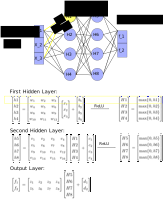
\includegraphics[width=0.5\textwidth]{mlp}
	\caption{A simple Feed Forward ANN with two hidden layers. This figure illustrates a graphical model for Equation \ref{mlp_eq} - 3.3 as well as explicitly showing the matrix operations performed by the different neurons on a single vector input. The output dimension is set arbitraily to be a $2\times1$ vector, which could for instance be used as class scores in binary classification; in practice, the dimension will be problem dependent.}
	\label{fig:mlp}
\end{figure}

The ANN model we have described thus far is known as Feedforward Network or a Fully Connected Network, which refers to all neurons being connected to all other neurons in the preceding and succeeding layers. This is an important point as it fascilitates a hierarchical structure in which neurons in the later layers may combine features from earlier layers to create more complex features in turn. Relatedly, this architecture enables distributed representation in which several types features can be combined in different ways to represent an exponential number of different inputs \cite{Hinton1985}. As an example, if we had squares, rectangles and circles and each of them could be either red, green or blue, then we have 9 possible visual objects, yet all the possibilities could efficiently be represented by combining three color neurons with three shape neurons \cite{Goodfellow2016}. \textbf{see goodfellow ch 15}.

\subsection{Training ANNs}

In a typical classification problem we have $n$ possible labels for each input and wish to predict a probability distribution over them. In these applications the outputs of ANN are transformed into 0 to 1 range. More formally, consider that the output from above ANN for a single input $\mathbf{x}$ is the $n \times 1$ vector $\mathbf{f}$; we then require, that each element of $\mathbf{f}$ is between 0 and 1 and that $\sum_1^n \text{f}_i = 1$. The most common way of doing this is to assume that the output of the ANN are unnormalized (predicted) class log-probabilities, that is $f_i = \log \hat{P}(y = i | \mathbf{x})$ \cite{Goodfellow2016}. By taking exponents and normalizing across possible labels predicted class probabilities are calculated as per below - this is known as the softmax function:

\begin{align} \label{softmax_eq}
  \text{softmax}(\mathbf{f})_i = \frac{\exp (f_i)}{\sum_j \text{exp}(f_j)}=q_i
\end{align}

where $q_i \in [0,1]$ captures the predicted probability that the input into the ANN belongs to class $i$. One reason for the softmax layer's popularity is that it is easily compatabile with the cross entropy loss function defined as $L_i=-\sum_i p_i \log q_i$ \cite{Shannon1948}. In simple image classification tasks where the classes are mutually exclusive we have $p_i=0 \forall i\ne C$ and $p_i=1$ for $i=C$ denoting the correct class. Plugging Equation \ref{softmax_eq} into this equation gives:

\begin{align} \label{XEloss}
  L_i  = -\log \left(\frac{\exp (f_C)}{\sum_j \text{exp}(f_j)}\right) = -f_C + \log\left(\sum_j \text{exp}(f_j)\right)
\end{align}
which is the loss incurred from one observation, and is clearly continuous and differentiable. The sequence of computation leading from model inputs all the way to the output of scalar loss is known as the forward pass. Usually forward pass is computed simultaneously for several inputs, known as a mini-batch, in which case the average loss across the mini-batch is typically used. 
The aim of training an ANN is based on learnng model weights that minimize some appropriate loss function, such as the cross-entropy loss above. Most supervised deep learning models, including the basic feedforward-network described above, are nowadays trained using the back-propagation algorithm \cite{Linnainmaa1976} \cite{Rumelhart1985}. The main idea of this algorithm is to use the chain rule to decompose the gradient of a loss function so that it can be efficiently passed back through the network. More formally, assume the loss of an ANN is produced by a sequence of $m$ nested operation:

\begin{align} \label{bp_eq1}
  L(y_i, x_i) = f^{(m)}(y_i, f^{(m-1)}(\dots f^{(2)}(f^{(1)}(x_i))))
\end{align}
where $y_i$ is the real label of the observation, $x_i$ the input data, the different $f^{(i)}$ may for example represent different types of layers. Employing the chain rule recursively, a simple decomposition gives:

\begin{align} \label{bp_crule}
  \frac{\partial L}{\partial x_i} = \frac{\partial L}{\partial f^{(m)}}\frac{\partial f^{(m)}}{\partial f^{(m-1)}} \dots \frac{\partial f^{(1)}}{\partial x_i}
\end{align}

These computations are done in the opposite order of the forward-pass operations; hence back-propagation. Above example is simplistic since usually in addition to inputs from preceding layer, each layer has also its own paramets which can be also be thought as inputs to that layer. The general idea of the chain rule still works in that situation as well, now however the gradient flow bifurcates at each layer; part of gradients flow into tha earlier layer while the others flow back into parameters; this is explained in more depth in Figure \ref{fig:backprop}. By representing ANNs as computational graphs, and using the chain rule similar to above, it becomes easy to see how backpropagation can be used to send appropriate gradients to right places even in complex network architectures. Importantly, backpropagation does this efficiently since at each operation all upstream gradients are collated and then passed on to one layer down, which is a lot more efficient than considering every single path through an ANN individually. To see this, consider Figure \ref{fig:mlp}: using back-propagation we can start from the output and, for instance, calculate the derivative of the output layer with respect to $H5$ neuron only once, and then pass this derivative to all neurons $H1$ - $H4$ simultaneously, which requires a lot less computation than considering all the paths that involve $H5$ separately. 

\begin{figure}
  \centering
	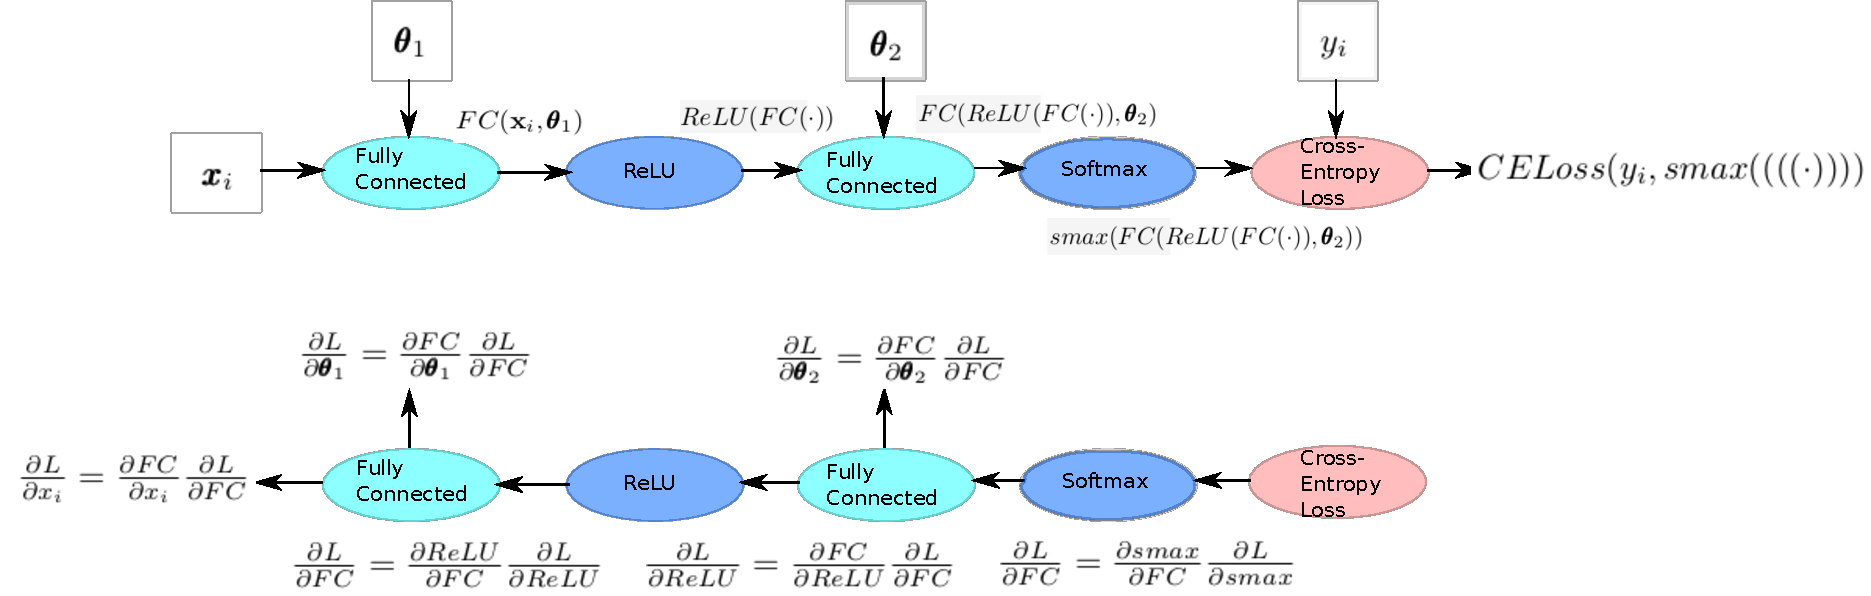
\includegraphics[width=\textwidth]{backprop}
	\caption{A simple example of forward (top) and backward passes (bottom) for a simple two-layer ANN, which illustrates how gradients flowing to early layers are calculated by multiplying the local gradient of a given layer with the gradient that flows back from the next layer}
	\label{fig:backprop}
\end{figure}

After gradients are calculated using back-propagation, they are used by an optimization algorithm to change the model's parameters with the aim of minimizing the loss function. Here we consider stochastic gradient descent (SGD) \cite{Robbins1951} which is likely the most widely used optimization algorithm in deep learning. This algorithm is called stochastic because at each learning iteration only a subset, known as mini-batch, of the data is use to calculate gradients and to perform parameter updates; it has been shown that SGD converges much faster than calculating gradients always on all available data; the time per update for the algorithm is independet of size of data as long as batch size is held constant \cite{Goodfellow2016}. The parameter updates are based on moving 'downhill' i.e. in the direction of negative gradients:

\begin{align} \label{sgd_eq}
  \pmb{\theta}_{(t+1)}=\pmb{\theta}_{(t)} - \eta \nabla_{\theta_{(t)}}L(\mathbf{X}, \mathbf{y})
\end{align}

Most deep learning models are very sensitive to the choice of learning rate $\eta$; if it is too high, we are likely to miss minima and conversly there is a risk of local minima and slow training time when the parameter is set too small. Usually learning rate is reduced linearly with training, or in bigger steps at regular intervals, to reduce the impact of noise when we are near a minimum \cite{Goodfellow2016}.

Another common addition to the vanilla SGD is momentum \cite{Rumelhart1985}, which can accelerate learning when there is a lot of noise from SGD or when the Hessian of the loss (matrix of 2nd order derivatives) is ill-conditioned as shown in Figure \ref{fig:momentum}. SGD with momentum ammends the original SGD by introducing a velocity term that accumulates gradients from previous iterations with an exponential decay. Rumelhart and Hinton \cite{Rumelhart1985} described momentum as if dropping a ball-bearing on loss surface and letting momentum drive the ball. Further, the loss landscape can be imagined to be immersed in a liquid with a specified level of viscosity that defines how quickly the momentum fades. Algorithm \ref{alg:sgd_mom} gives an example of full SGD momentum algorithm for learning model parameters. In practice, back-propagation and optimization can nowadays be done automatically by modern deep learning libraries such as PyTorch \cite{Paszke2017} and Tensorflow \cite{Abadi2015}. 

\begin{figure}
  \centering
	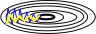
\includegraphics[width=0.5\textwidth]{momentum}
	\caption{Example of ill conditioned Hessian and how momentum speeds up learning by accumulating the gradients of previous iterations such that velocity towards centre (lower loss) is established (shown in yellow). SGD without momentum keeps jumpin across the loss surface as if in a downward sloping canyon, but failing to utilize the slope (blue trace). The contours depict different levels of loss that decreases inwards}
	\label{fig:momentum}
\end{figure}

\begin{algorithm}
  \caption{SGD with momentum (following \cite{Goodfellow2016})} \label{alg:sgd_mom}
\begin{algorithmic}
  \Require Learning rate $\eta$, Momentum decay parameter $\alpha$
  \Require Initial parameters $\pmb{\theta}$, initial velocity $\nu$
  \While{Convergence not met}
  \State Sample a minibatch of m observations from training data $\{\mathbf{x}_1, \dots, \mathbf{x}_m \}$ and their
  \State Get corresponding targets from training data $\{\mathbf{y}_1, \dots, \mathbf{y}_m \}$ 
  \State Compute gradient for the minibatch: $\mathbf{g} \leftarrow \frac{1}{m} \nabla_{\theta}\sum_i L(f(\mathbf{x}_i| \pmb{\theta}), \mathbf{y}_i)$
  \State Update velocity: $\pmb{\nu} \leftarrow \alpha \pmb{\nu} - \eta\mathbf{g}$
  \State Updata parameters: $\pmb{\theta} \leftarrow \pmb{\theta} + \pmb{\nu}$
  \EndWhile
\end{algorithmic}
\end{algorithm}

\subsection{Convolutional Neural Networks (CNNs)}

So far we have considered only simple feedforward ANNs with fully connected layers. Most of the ground-breaking accomplishments over the past decade in deep learning have however been achieved with convolutional neural networks (CNNs) \cite{Le} of some sort. This is particularly true for computer vision tasks such as image classifiction \cite{JurgenSchmidhuber2015}. In fact, the term deep learning is often used synonymously with CNNs that have a large number of layers.

Unlike fully connected neurons in feedforward networks, convolutional layer has neurons, usually called kernels, which are connected only to some parts of the input it receives from its preceding layer - together many such neurons span the entire input data. Furthermore, there is weight sharing between the kernels to allow for the recognition of a particular feature anywhere in the input space \cite{Lecun2015}; convolution layers are thus particularly suited for data with locally correlated structures such as images. Consider an input image of 225x225, a typical convolution filter may have size 3x3 and, after having been trained on image data, could have learnt feature mapping that represents particular visual feature such as a vertical edge. This filter is then replicated over the entire 225x225 input range so that the model can detect that particular feature anywhere in the image. Usually each layer has a multitude of such kernels to detect different features in the input data. Mathematically, this feature detection corresponds to the convolution operation between input data $X$ and convolution kernels $K$, which for discrete 2D data is given as $S(i, j) = (X \ast K)=(i, j) \sum_m \sum_n X(i-m, j-n)K(m, n)$ \cite{Goodfellow2016} where $i$ and $j$ denotes a particular image pixel location and $m$ and $n$ those of the kernel. Figure \ref{fig:conv} gives a brief toy example to illustrate this process. 
  
\begin{figure}
  \centering
	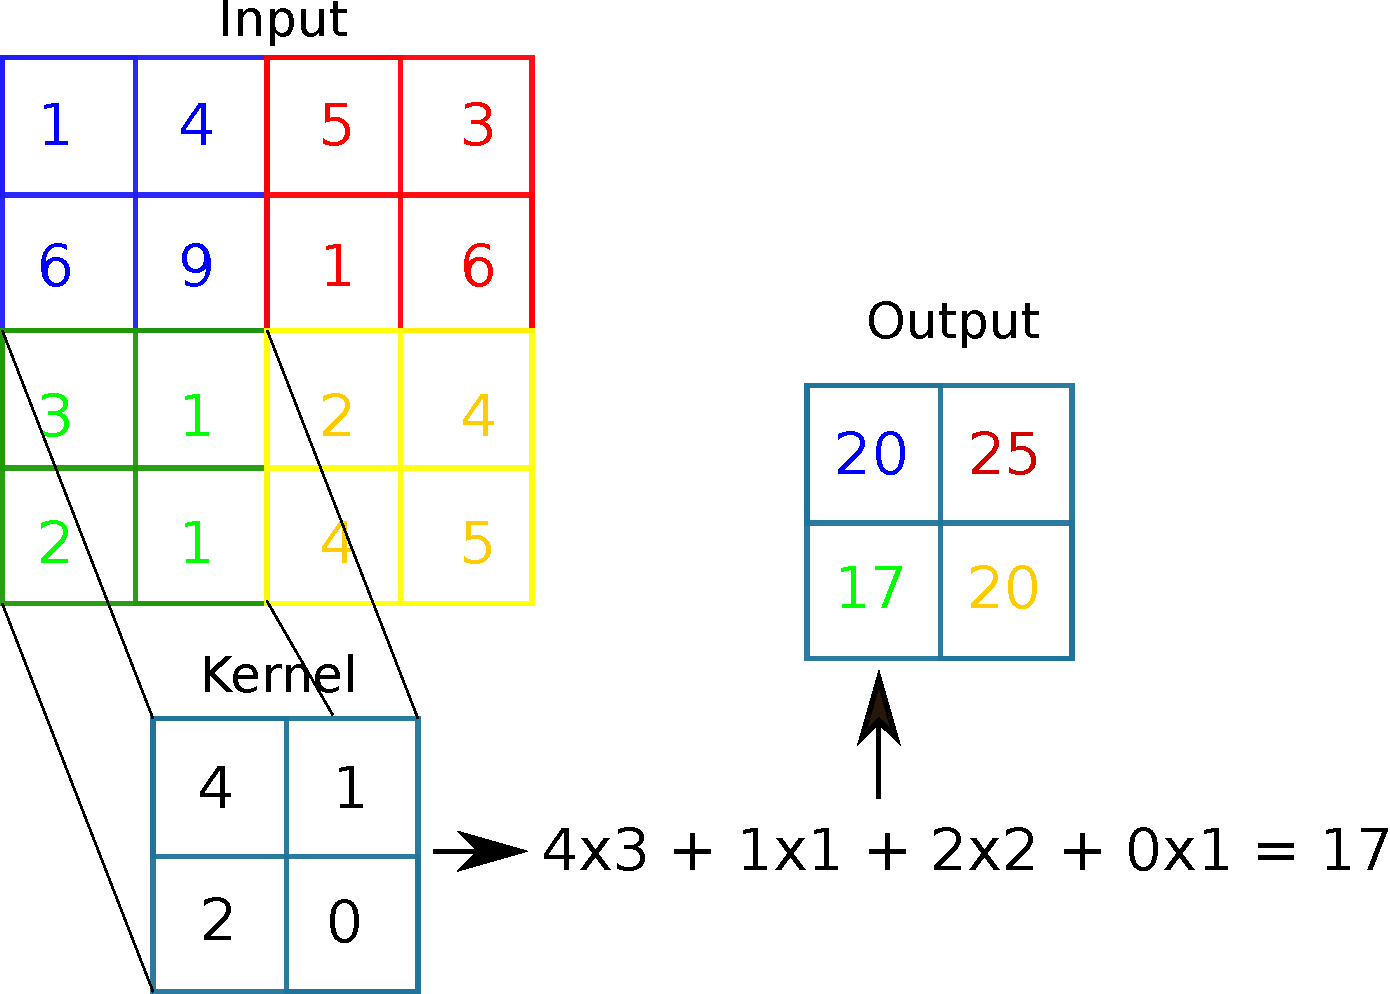
\includegraphics[width=0.7\textwidth]{conv}
	\caption{A simple example of the computations performed by a single 2x2 convolution kernel on a 4x4 input. Assuming stride length of two squares, the kernel will see each of the four corners and performs a convolution operation on each of them. This is shown explicitly for the bottom left green square. The computation is hence essentially a dot product similarity metric between the kernel and the local image areas.}
	\label{fig:conv}
\end{figure}

The reason why convolutions have proved so effective for image data is that natural visual scenes present strong local correlations - the world we view is not just a collection of randomly ordered pixels. Additionally, these visual features can appear at essentially anywhere in our visual scenes; thus the need for convolution layers to scan across the whole image \cite{Lecun2015}. Further, CNNs usually have several layers of convolutions on top of each other. When such deep CNNs are trained on image data, the kernels across the different layers usually learn a hierarchy of visual features, such that the early layers detect edges and corners, which are then used by middle layers to create contours and parts of objects, and finally later layers build up more complex representations, possibly of complete objects \cite{Zeiler2014}. This shares some similarities with mammals' visual cortex \cite{Cadieu2014} in which earlier (V1) cells respond to edges and bars of different orientations \cite{Hubeld1962} and later ones like V4 and the IT cortext to more complex shapes \cite{Kobatake1994}. This idea of distributed hierarchical representations is crucial to our research. First, the abiliy to learn fundamental visual features, such as edges, should help to generalize models to novel visual scenes. Second, generalization is also improved by hierarchy of features: for example, if a CNN only trained on images of cats and apples, is shown a picture of a dog, it would be more likely to classify it as a cat than apple which is arguably the closer of the two. In the next chapter we show how an extension of this idea can be explotited to perform more accurate predictions for previously unseen classes of objects.

Convolution layers in CNNs are normally followed up by max-pooling functions. Usually this is just the $max()$ function applied to a grid output of its preceding convolution output. For example, in Figure \ref{fig:conv} the max-pooling would only pass through the value of 25. The benefit of such down-samplign is local invariance: visual objects are not completely rigid and by passing on only the largest value, we are likely to produce the same output even if the values of the square changed around a bit \cite{Lecun2015} (imagine a letter that's slightly rotated between different views).

One of the most important features of CNNs is that they can be trained end-to-end using back-propagation and SGD. A consequence of paramount importance is that the type of visual features which convolution kernels learn to represent is fully determined by what best fits the data, and they can be learned directly from raw data. This is in sharp contrast to earlier computer vision image classification that usually involved feature extraction techniques \cite{Prince2012} such as SIFT \cite{Lowe1999} in which manually designed features are used. These features would then be passed to a separate classifier, for example Support Vector Machine \cite{Weston2010}. CNNs with their automatic feature learning capability produced very large accuracy gains on this apprach \cite{Razavian2014} and following the breakthrough performance of the seminal AlexNet CNN \cite{Krizhevsky2012} at the ImageNet 2012 competition, deep CNNs of various designs have become state-of-the-art in virtually all machine vision classification and detection tasks \cite{JurgenSchmidhuber2015}.

In addition to convolution and pooling layers, CNNs involve several other important architectural designs. For example, deep networks with a large number of convolution and pooling layers have been found to perform better \cite{Srivastava2015} than shallow ones. This is exploited by several CNN models such as the ResNet architectures which can have more than 100 layers \cite{He2015}. Theoretically, depth increases the representational capacity of the network \cite{Sun2015}. Representational capacity is also increased by the use of ReLUs on top of convolution layers. All in all, modern deep CNNs can easily have hundres of millions of parameters and the ability to learn super-human performance on many image classification tasks \cite{Lecun2015}. Due to their large representational capactiy, these models can also easily overfit training data and the development of appropriate regularization techniques has played a large role in CNNs recent achievements. Perhaps the most popular regularization technique, and the one applied in this work, is DropOut \cite{Srivastava2014}. During model training, dropout deactivates a each neuron in each iteration with a probability $P$. The consequence of this is that over the entire training period we essentially end up training an ensemble of different models, and the final model is an average of exponentially many sub-models \cite{Goodfellow2016}. This method regularizes the network as individual neurons can not rely too much on any other neurons and the output expected to get out of them. Durng test-time, dropout is turned off.

Many of the theoretical concepts of modern deep CNNs have been around for several decades \cite{JurgenSchmidhuber2015}. The reason for their recent surge in popularity is to a large extent that they have become a lot easier and faster to train as our computers have gotten more powerful and our datasets much larger. In particular, the ability to train deep models on Graphical Processing Units (GPUs) has cut training times by at least an order of magnitude \cite{Lecun2015}. However, we have only been able reap the benefits of faster compute and better models because of 'big data'. It has been suggested that CNNs with around 5000 labels per training category can on average start to match human performance \cite{Goodfellow2016} - over the past decade we have seen the advent of datasets that have up to tens of millions of training examples \cite{Russakovsky2015i}, \cite{JiaDeng2009}, \cite{Netzer2011}.

\section{Exploiting Semantic Information in \\ Computer Vision}

\subsection{Semantic Hierarchies and \\ the Human Visual System}
Upon observing almost any visual scene, humans are able to effortlessly cut it up into segments of distinct objects \cite{Rosch1976}, even if we have never seen the scene before. This is a remarkable ability considering that the world we live in can present us with an infinite amount of visual variation to our retinas and yet we are able to easily recognize tens of thousands of distinct object categories \cite{Biederman1989} with invariance to various factors such as movement, lighting, shade, orientation and partial occlusion \cite{DiCarlo2012}. Rosch \textit{et al.} \cite{Rosch1976} argue that this is because of the non-random, and hierarchical, structure of visual objects, for instance no breed of dogs will have wings but they will often share many features such as four legs with certain type of paws. In general entities that are closer to each other in a hierarchical semantic taxonomy will also typically share more visual features; dogs and birds are still more alike than dogs and vehicles since both belong to a higher level category of animals which all share certain visual attributes. Deselaers and Ferrari \cite{Deselaers2011} veried these observations in their study on the visual separability of different semantic categories using the ImageNet dataset.

Standard machine learning and deep learning models used for image classification do not exploit this semantic taxonomy since they are typically trained against one-hot encoded target vectors. For example, the 1K ImageNet data set \cite{JiaDeng2009} will have labels as 1000-dimensional vectors where there is 1 for the dimension indicating the correct class and zeros elsewhere. It follows that label vectors for different classes are thus orthogonal and normally a model trained on this data will therefore not account for any classes belonging to a common category at a higher level of the taxonomy. For example, in reality two different breeds of dog do fall under the same higher level categories of dogs, animals, mammals and so forth - all of these share certain amount of visual features. The chosen level of hierarchy of a one-hot encoding is also usually arbitrary; should an image be labelled a dog or a labrador retriever? Optimally both would be taken into account, we argue. The number of machine learning algorithms that do take this into account is limited, however; below we give an overview of them.

\subsection{Semantic Hierarchies for Image Classification}
The use of semantic hierarchies in computer vision dates back to early work on image retrieval \cite{Aslandogan1997}, \cite{Zhao2001}, \cite{Grosky2002} \cite{Barnard2001}, where it has been used to expand potential query terms and to impose a more general association between image features and corresonding labels. These ideas were subsequently utilized to improve image annotation and classification \cite{Srikanth2005}, \cite{Marszaek2007} \cite{Griffin2013}. For example, Marszalek and Schmid \cite{Marszaek2007} use the WordNet database to create a lexical hierarchy of their image labels and train an SVM classifier \cite{Scholkopf2002} that acts at each node of the hierarchy. The resulting model proves very flexible and performs well under uncertainty - if the model is unsure about what dog breed is in an image, it can then move up one level and just predict a 'dog'. It should be noted that the dataset used by the authors is very simple by today's standards, however. More recently, Redmon and Farhadi \cite{Redmon} employed a similar idea but in the context of deep learning. In particular, for each image, its label was taken to be the full path from the root node of the WordNet tree to the originl singular label. The model was then trained with multiple softmax functions, one for each level of hierarchy in order produce a chain of conditional probabilities from the root node to leaves. The authors' purpose for building this model was to learn simultaneously from two datasets of unequal hierarchies and to jointly optimize classification and detection (locating an object) on the two datasets. However, other possible benefits of such a flexible model, like generalization to new classes, were not explored in detail. 
In their research on human categorization, Rosch \textit{et al.} \cite{Rosch1976} defined the concept of 'basic level'. This is described as the most fundamental level of a specific category in the semantic taxonomy and is the one first learnt usually by children and also objects are identified the quickest at this level. The level below basic level is called 'subordinate level'. An example of this structure would be the basic level label of 'fox' and its subordinate 'arctic fox'. The importance of the basic level seems to stem from this level having the highest ratio of visual variation between categories to variation within categories \cite{Rosch1976}, \cite{Joliceur1984}. It results that it has been especially practical for humans to identify and label objects at this level. 

Hillel and Weinshall \cite{Hillel2007} implemented the idea of basic and subordinate levels by building a two-stage classifier where the first stage generates a vector representing the different parts of an objects and the second stage classifies instances based on this vector. On average, this strategy outperformed a traditional one-step algorithm. Wang and Cottrell \cite{Wang2015} took these ideas to the deep learning-era an trained a CNN on both basic and subordinate labels of the ImageNet 2012 data \cite{Russakovsky2015}. They found that this leads to an improved performance on the standard top-5 classification accuracy. Another simiar study \cite{Lei2018} explored a dataset which mostly had coarse labeled images (similar to the basic level) and only some fine grained examples. The authors showed that their custom CNN, which used both hierarchies, could predit fine-level labels better than a model that's only trained on fine level. This suggests that the fine-grained model is able to borrow strength from coarse labels and consequently generalize better. Peterson \textit{et al.} extended this line of research by exploring the type of representations learnt by a CNN trained on both 'basic' and 'sub-ordinate' labels. First, the authors found that including the basic-level labels in pre-training or fine-tuning led to a much more clustered representation of the feature spaces extracted from the final layer of the CNN (e.g. the features vectors of different breeds of dogs were now bundeled up together whilst if trained on just subordinate labels, then there was no clustering of similar categories). The features also had learn separate hierarchies for natural and man made objects. Finally, they illustrated the generalization power of these representations by running a zero-shot learning experiment in which the model was shown only a few examples of either sub- or basic-level objects and then tries to find all other images from the data set belonging to the given label. Interestingly, the results show that the supplementary basic-level training had led to a bias to label objects at this level which is congruent with corresponding studies in humans \cite{Xu2000}.

Despite the important contribution of above works, they are limited in that they only consider two levels of a semantic taxonomy. It has been shown that, despite the importance of the basic level, humans posses and utilize a much more complex multi-level semantic hierarchy \cite{Joliceur1984}. We are not aware of any deep learning papers that explore the type of representations and the consequent generalization properties that would be learnt by considering a multi-level semantic taxonomy. We attempt to fill this void by exploiting a full set of hierarchical taxonomy via semantic embeddings built on a large-scale lexical database WordNet \cite{Princeton2010}.

\subsection{Semantic Embeddings and Zero-shot Learning}
Above studies illustrate the implicit connection between text and visual data processing in humans. Joliceur \textit{et al.} \cite{Joliceur1984} explored the dependence of our visual system on semantic understanding in more depth and illustrated this with several experiments. For instance, upon viewing a picture of a chair we can use our semantic knowledge base to generalize it to the category of furniture even though the image itself doesn't reveal that such an abstraction even exists. Similary, we can seamlessly access our visual memory to imagine semantic concepts, even ones we may never have seen such as 'a cat wearing ice skates'.

Zero-shot learning (ZSL) \cite{Palatucci2009} is concerned with making predictions about previously unseen classes of images. Formally if a classifier $f$ is trained on features $X_{TR}$ and training labels $Y_{TR}$ such that $f:X_{TR} \rightarrow Y_{TR}$, then in ZSL for the possible class labels we have that $Y_{TR} \cap Y_{ZSL} = \emptyset$ where $Y_{ZSL}$ represents the test labels of any ZSL dataset. A fundamental idea in this area was to exploit the semantic relatedness of visually linked categories \cite{Monay2004}, \cite{Weston2010}, \cite{Palatucci2009} by projecting input data into a lower dimensional semantic embedding space. This can be represnted by the following equations \cite{Palatucci2009} (see Figure \ref{fig:zsl} for a graphical explanation):
\begin{align} \label{zsl_eq}
  \mathcal{S} &: X^d \rightarrow F^P \\
  \mathcal{L} &: F^P \rightarrow Y
\end{align}
Here we assume that we have a full collection of all pairs $\{f, y\}_{1:M}$ of both seen and unseen classes where $f$ is the point in the semantic embedding space $F^P$ that corresponds to the label $y$. In the training phase we can take the data for the seen classes $\{X, y\}_{1:N}$, where $N<<M$, and replace each $y$ with its embedding vector $f$ and thus learn the mapping $\mathcal{S}$. Labels for objects of unseen classes can then be predicted by first mapping them into $F^P$ through $\mathcal{S}$ and then employing $\mathcal{L}$ to find the most appropriate $y$ based on the predicted semantic embedding; this could for instance be a nearest neighbor classifier. The trick is thus having the semantic embedding space $F^P$ to contain vectors for all seen and unseen classes. To be clear, the term 'zero-shot' thus refers to the trained model never having seen $M-N$ of the classes but in our semantic knowledge base we do know about the existence of those zero-shot classes and their names. The challenge is thus in how to construct the semantic embedding space and what type of model to use to learn $\mathcal{S}$; the following paragraphs will cover the existing approaches.

\begin{figure}
  \centering
	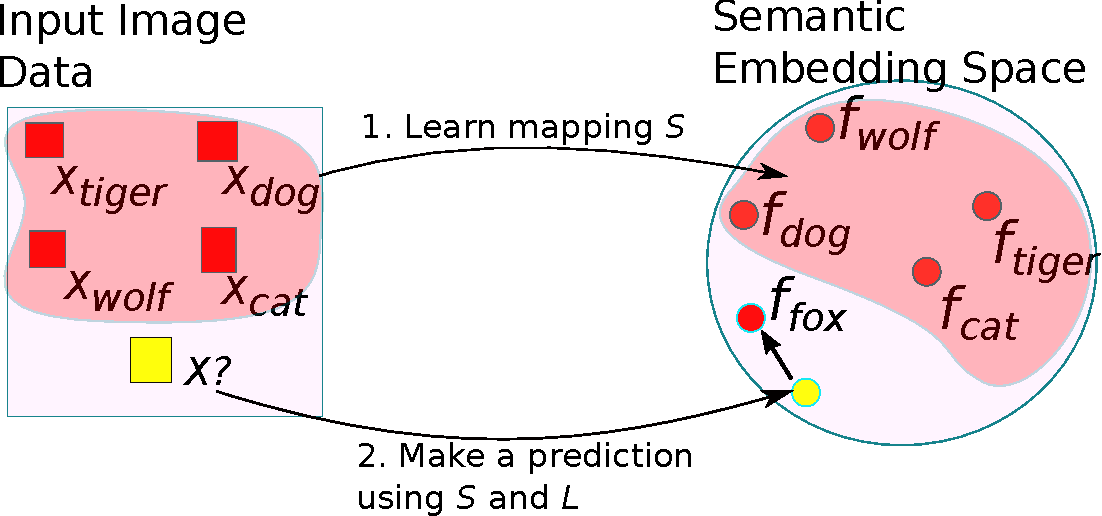
\includegraphics[width=\textwidth]{zsl}
	\caption{A graphical illustration of zero-shot learning where the left square contains all input images. Red ones are the training classes whcih are used to learn a mapping $\mathcal{S}:X^d \rightarrow F^P$. The circle represents the semantic embedding space. Note how we can access embedding vector for also classes we dont have visual training data for. Upon seeing a novel image (yellow square) we predict its embedding vector (yellow dot) and then find nearest plausible classe (here fox) using some function $\mathcal{L}$. Novel image is hence classified as a fox even though the model has never seen one before}
	\label{fig:zsl}
\end{figure}

In one of the early works on the topic, Socher \textit{et al.} \cite{Socher} created word embedding vectors for all seen and unseen class labels from freely available Wikipedia data using a methodology \cite{Huang2012} that uses local and global context of the words to place similar words next to each other in the embedding space. A two-layer feedforward network was then used to learn a mapping from images features into the embedding manifold. Outlier detection was used to determine if the predicted embedding was one of the known or unknown classes. Only 8 known classes and 2 unknown classes were considered however. To address this and other limitations, Frome \textit{et al.} \cite{Frome2013} developed the Deep Visual-Semantic Embedding Model (DeViSE), which was trained on 1000 classes of the ImageNet dataset and its ZSL abilities were tested on the remaining 20,000 classes. This model structure is similar to ours in that it takes a pre-trained deep learning model, AlexNet (which won the 2012 ImageNet competition) \cite{Krizhevsky2012}, and then removes the softmax layer and replaces it with a projection layer that attempts to predict the word vector embedding of each image label. The word embeddings, in turn, were extracted from a skip-gram model trained on 5.4billion words of text from Wikipedia. The skip-gram model \cite{Mikolov2013}, \cite{Mikolov} learns to place vectors of similar terms near to each other by attempting to predict adjacent words. This model succesfully used the semantic information to make correct guesses on thousands of unseen classes, and it still provides a good baseline for new methods as we will show in our results section. 

The authors of DeViSE worried however that the model was overfitting the transformation from the image representations into the semantic feature space. To overcome this they introduced another novel model called Convex Combination of Semantic Embeddings (ConSE) \cite{Norouzi2013}. The idea is as follows: take a previously unseen image class and simply feed this into a pretrained deep learning model which has been trained on, say 1000 classes. The model will consequently try to predict this new image as one of the known thousand classes and outputs respective 1000 predicted class probabilities $p_0 (y | \mathbf{x})$ such that $\sum_{y=1}^{1000} p_0 (y | \mathbf{x}) = 1$. The predicted semantic embedding for the new class can then be taken as the convex combination of the known classes weighed by the predicted probabilities from the previous step. More formally \cite{Norouzi2013}:
\begin{align}
  f(x) = \frac{1}{Z}\sum_{t=1}^T p(\hat{y}(\mathbf{x}, t)| \mathbf{x}) \cdot \mathcal{L}(\hat{y}(\mathbf{x}, t))
\end{align}
where $\hat{y}(\mathbf{x}, t)$ is the $t^{th}$ most likely class-label for image $\mathbf{x}$ out of the known labels, with $p()$ giving the respective probability. $\mathcal{L}$ maps each of these labels deterministically to their embedding. $Z$ is a normalizing consant, and $T$ is user-defined. This model was shown to generalize slightly better to novel classes than DeViSE when both used the same image features and embedding vectors. 

A potential problem with using wikipedia to create embeddings in the ConSE model above is that vectors for low occurence labels may be imprecise. Li \textit{et al.} attempt to resolve this by using the full WordNet hierarchy. For example, the semantic embedding for the word 'arctic fox' is constructed as a distance-weighted combination of the semantic embeddings of the hypernym (parent) nodes in the WordNet ('arctic fox', 'fox', 'canine', 'carnivore' and so on) up to the root. Whilst this improved the performance over the ConSE model, the semantic embedding for each node in the WordNet hierarchy still comes from a source that does not account for this taxonomical structure. Further, each label only considers its own parent nodes. Consequently the resulting embedding manifold in Euclidean space is unlikely to accurately reflect the entire WordNet graph and its complex relations. In the next section we show how this can be achieved with Poincare embeddings.

Over the past few years we have seen several other important contributions to the area of ZSL. Most works learn semantic embedding and the mapping function separately, however Ba \textit{et al.} \cite{Ba2015} train a feedforward network from text features that is able to predict the visual features in the different layers of a CNN and thus learns a good embedding. 

Changpinyo \textit{et al.} \cite{Changpinyo2016} on the other hand consider a weighted graph of semantic embeddings in one manifold and align this with a weighted graph of possible model weights in another manifold by projectin graph vertices. So called phantom classes are learned to optimally connect seen and unseen classes in the graphs on the basis of the semantic space, and classifier for unseen classes are constructed as the convex combination of phantom classes in the model space. 



Ji \textit{et al.} \cite{Ji2017} show how performance can be improved by ensuring that the embedding manifold preserves the local structure of the visual input space, thus encouraging visually similar classes to be closer to each other in the embedding space. The authors also highlight and suggests a solution to the project domain shift problem, that is, the learned mapping from seen images to the embedding space may not transfer well to the unseen classes.  Tsai \textit{et al.} \cite{Tsai2017} use two autoencoders, one on just the image data and another on text data, extract the representation layer from each and minimize their mismatch. The advantage of this model is that the unsupervised nature of autoencoders allows both labeled and unlabeled data to be used and thus more robust representations to be learnt. Zhang and Saligrama \cite{Zhang2015} build semantic embedding labels for unseen classes as mixture distributions of the embedding vectors of the seen classes. These are employed during test time to find the closest match for the mixture distribution of the test image. In a follow up work the authors \cite{Zhang2015a} provide a latent probabilistic framework in which zero-shot recognition is performed by estimating the posterior probability that the test image matches one of the label vectors. 

Fu \textit{et al.} \cite{Fu2015} identified the issue of the projection domain shift that exists with most ZSL model, that is, the mapping that is learned from the image space into the embedding space may not transfer well to the disjoint set of unseen classes. Transductive multi-view embedding is proposed as a solution: in addition to training data, multiple semantic embeddings of each test labels are used in training phase as well, with all of them projected onto a common embedding space. See also Rohrbach \textit{et al.} for similar ideas \cite{Rohrbach2013}. The use of test labels during training may not be practical however, and as an alternative Kodirov \textit{et al.} \cite{Kodirov2017} propose a semantic autoencoder as a solution to this problem. The general idea of these autoencoder is to learn a mapping from images to semantic embedding space (encoder) and a mapping from the embedding back to input to reconstruct it as well as possible (decoder). The addition of the decoder constraints the model to solve the domain shift.


Shigeto \textit{et al.} \cite{Shigeto2015} show that instead of learning a mapping from images to label space, it can be beneficial to learn this mapping in the opposite direction since nearest neighbor search is often easier in the lower dimensional image space. This however assumes high dimensional embedding vectors, which we manage to avoid as we employ hyperbolic spaces. Zhang \textit{et al.} utilize a similar idea alongside CNNs.

Fu and Sigal \cite{Fu2016} introduce the idea of using embeddings built on full semantic vocabularies rather than just training labels in order to learn a better mapping between image and semantic embeddings. 

Fu \textit{et al.} \cite{Fu2015a} note that the vectors embedded in a semantic space often form class manifolds. Motivated by this observation they build a semantic manifold graph out of the labels in the embedding space and create a special form of a markov chain process that predicts the unseen class label.


There also a plethora of models that focus on zero-shot learning via class attributes \cite{Xian2016}, \cite{Romera-Paredes2017}, \cite{Bucher2016}
A limitation of these is when number of classes grows very big however the set of attributes is harder to manage manually, instead we prefer to learn similarities in the embedding spaces. More recently attribute based zero-shot has mainly been motivated by wishing to predict fine-grained classes that are visually very similar \cite{Xian2016} \cite{Reed2016} our motivation is different however as we are focusing on model that generalizes well on a large-scale. The set of attributes is also hard to transfer to new context \cite{Ba2015}. Manually defined attribute taxonomy is required\dots

Finally, some works combined semantic embeddings and attributes \cite{Akata2015}, \cite{Fu2015} \cite{Zhou2005}. Akata \textit{et al.} \cite{Akata2015} combine three embeddings, one learnt from the Wikipedia dataset, one for physical attributes of animals and a hierarchical embedding, which attempts to capture the taxonomical structure of the WordNet using various distance measures such as the shortest path between nodes. The model performs well on zero-shot prediction of fine-grained classes on a relatively small data set; it's generalization properties on a large data set such as the 21,000 label ImageNet are not explore however.  




\bibliographystyle{ieeetr}
\bibliography{Thesis}

\end{document}
